\documentclass[russian]{beamer}

% To be compiled with pdflatex
% (XeTeX's font is somewhat bigger (?), so on some slides the text does not fit into the slide borders)

\usepackage{mystyle}

\graphicspath{ {images/} }

\usetheme{Warsaw} % Warsaw Copenhagen Madrid CambridgeUs Darmstadt Frankfurt Singapore
\setbeamertemplate{headline}{}

\definecolor{beamer@blendedblue}{RGB}{0, 83, 83}  % 104
\definecolor{my-red}{RGB}{176, 0, 0}
\definecolor{my-blue}{RGB}{0, 0, 153}


% Inserting frame numbers in footline
% http://tex.stackexchange.com/questions/191198/customization-of-the-copenhagen-theme
\makeatletter
  \iffalse
  \pgfdeclarehorizontalshading[frametitle.bg,frametitle right.bg]{beamer@frametitleshade}{\paperheight}{%
    color(0pt)=(myblue2);
    color(\paperwidth)=(white)}
  \fi

  \defbeamertemplate*{footline}{mysplit theme}
  {%
    \leavevmode%
    \hbox{\begin{beamercolorbox}[wd=.5\paperwidth,ht=2.5ex,dp=1.125ex,leftskip=.3cm plus1fill,rightskip=.3cm]{author in head/foot}%
      \usebeamerfont{author in head/foot}\insertshortauthor
    \end{beamercolorbox}%
    \begin{beamercolorbox}[wd=.5\paperwidth,ht=2.5ex,dp=1.125ex,leftskip=.3cm,rightskip=.3cm plus1fil]{title in head/foot}%
      \usebeamerfont{title in head/foot}\insertshorttitle\hfill
      \insertframenumber\ / \inserttotalframenumber\hspace*{0.5em}
    \end{beamercolorbox}}%
    \vskip0pt%
  }
\makeatother


\setbeamertemplate{navigation symbols}{} % switch off navigation bar
\setbeamertemplate{itemize item}[ball] % Загадка, но без этого у itemize не будет кружочков
\setbeamertemplate{itemize subitem}[triangle]


% https://tex.stackexchange.com/questions/12735/can-one-replace-bullet-points-with-graphics
\newcommand{\labelitemi}{\usebeamertemplate{itemize item}{}}
\newcommand{\labelitemii}{\usebeamertemplate{itemize subitem}{}}


\AtBeginSection[]
{
  \begin{frame}
    \frametitle{Содержание}
    \tableofcontents[currentsection]
  \end{frame}
}


% https://tex.stackexchange.com/questions/530518/reset-footnote-counter-for-each-frame-in-beamer-class
\AtBeginEnvironment{frame}{\setcounter{footnote}{0}}


\title[Прямая ($2$D $+$ $3$D)]
{Семинар по аналитической геометрии: <<Прямая на плоскости (и в пространстве)>>}
\subtitle{}

\author[Василий А.]{
  Алексеев Василий
}

\institute[]
{
  %\textsuperscript{$\diamondsuit$}%
  МФТИ
}

\date[2020]
{
  \footnotesize{6 октября 2020}
}

\begin{document}

  \frame{\titlepage}
  
  \begin{frame}{Теория}
  
    \pause
  
    \begin{itemize}
      \item Векторное уравнение в параметрической форме:
        \begin{equation}
          \bds{r} = \bds{r_0} + \bds{a} t, \quad \bds{a} \not= \bds{0},\ t \in \RR
        \end{equation}
      
        \pause
        
        В общей декартовой системе координат:
        \[
          x = x_0 + \alpha t,\ y = y_0 + \beta t,\quad \alpha^2 + \beta^2 \not= 0
        \]
        
        \pause
        
        Каноническая форма:
        \[
          \frac{x - x_0}{\alpha} = \frac{y - y_0}{\beta},\quad \alpha \not= 0,\ \beta \not= 0
        \]
        
        \pause
      
      \item Нормальное векторное уравнение:
        \begin{equation}
          (\bds{r} - \bds{r_0}, \bds{n}) = 0, \quad \bds{n} \not= \bds{0}
        \end{equation}
        
        \pause
      
        Можно переписать как
        \[
          (\bds{r}, \bds{n}) = D, \quad \bds{n} \not= \bds{0}
        \]
    \end{itemize}
  \end{frame}

  \begin{frame}{Теория}
  
    Общее уравнение прямой в декартовой системе координат:
    \begin{equation}
      Ax + By + C = 0, \quad A^2 + B^2 \not= 0
    \end{equation}
    
    \pause
    
    \begin{itemize}
      \item Направляющий вектор $\bds a$ может быть выбран как $(-B, A)$.
      
      \pause
      
      \item Нормальный вектор в \textbf{прямоугольной} системе координат:
      \[
        (\bds a, \bds n) = -B \cdot n_x + A \cdot n_y = 0 \Rightarrow \boxed{\bds n \propto (A, B)}
      \]
    \end{itemize}
  
    \pause
    
    Расстояние от точки $A \hm= (x_1, y_1) \hm= \bds r_1$ до прямой $l$:
    \begin{itemize}
      \item с начальной точкой $\bds r_0$ и вектором нормали $\bds n$
      \[
        \rho(A, l) = \frac{\bigl|(\bds r_1 - \bds r_0, \bds n)\bigr|}{|\bds n|}
      \]
      
      \pause
      
      \item в \textbf{прямоугольной} системе координат, где прямая $l$ может быть задана уравнением $Ax + By + C \hm= 0$:
      \[
        \rho(A, l) = \frac{|Ax_1 + By_1 + C|}{\sqrt{A^2 + B^2}}
      \]
    \end{itemize}
  \end{frame}


  \begin{frame}{Теория}
  
    Общее уравнение прямой в декартовой системе координат:
    \[
      Ax + By + C = 0, \quad A^2 + B^2 \not= 0
    \]
    
    \begin{block}{Определение}
      Алгебраическая линия на плоскости:
      \begin{equation}\label{eq:algebraic-line}
        A_1 x^{k_1} y^{l_1} + \ldots + A_s x^{k_s} y^{l_s} = 0, \quad k_i, l_i \in \NN_{\geq 0}
      \end{equation}
      
      Степень уравнения (порядок алгебраической линии):
      \[
        \max{\Bigl\{k_1 + l_1, \ldots, k_s + l_s\Bigr\}}
      \]
    \end{block}
    
    \begin{block}{Теорема}
      Алгебраическая линия порядка $p$ на плоскости в \emph{любой} декартовой системе координат может быть задана уравнением вида (\ref{eq:algebraic-line}) порядка $p$.
    \end{block}

  \end{frame}


  \section{\uline{6.1(2, 3)}}
  
  \begin{frame}{\# 6.1(2, 3)}
  
    \begin{block}{Условие}
      \begin{enumerate}
        \setcounter{enumi}{1}
        
        \item $\bds r = \bds r_0 + \bds a t \xrightarrow{\?} [\bds r, \bds a] = \bds b$
        
        \item $[\bds r, \bds a] = \bds b \xrightarrow{\?} \bds r = \bds r_0 + \bds a t$
      \end{enumerate}
    \end{block}
    
    \pause
    
    \begin{block}{Решение}
      \begin{enumerate}
        \setcounter{enumi}{1}
        
        \item
          \[\bds r - \bds r_0 = \bds a t
            \Leftrightarrow (\bds r - \bds r_0) \parallel \bds a
            \Leftrightarrow [\bds r - \bds r_0, \bds a] = \bds 0
          \]
          \[
            [\bds r, \bds a] = [\bds r_0, \bds a] \equiv \bds b
          \]
          
        \pause
        
        \item
          \[
            [\bds a, \bds b] = \bds a \times (\bds r \times \bds a) = \bds r (\bds a \cdot \bds a) - \bds a (\bds a \cdot \bds r)
          \]
          \[
            \bds r = \frac{[\bds a, \bds b]}{|\bds a|^2} + \frac{\bds a}{|\bds a|}\left(\frac{\bds a}{|\bds a|} \cdot \bds r\right)
            = \frac{[\bds a, \bds b]}{|\bds a|^2} + \bds a t
          \]
      \end{enumerate}
    \end{block}
  \end{frame}
    
    
  \section{5.17}
  
  \begin{frame}{\# 5.17}
    \begin{block}{Условие}
      Треугольник.
      Две медианы: $x \hm+ y \hm= 3$ и $2x \hm+ 3y \hm= 1$.
      Вершина $A(1, 1)$.
      Уравнения сторон?
    \end{block}
    
    \pause
    
    \begin{block}{Решение}
      \begin{enumerate}
        \item Вершина не лежит на медианах: $1 \hm+ 1 \hm{\not=} 2$, $2 \hm\cdot 1 \hm+ 3 \hm\cdot 1 \hm{\not=} 3$
        
        \pause
        
        \item \emph{Пусть} $B$~---~вершина, соответственная медиане $x \hm+ y \hm= 3$
        
        \pause
        
        \item
        Пусть $M_{AC}$ и $M_{AB}$~---~середины сторон $AC$ и $AB$ соответственно:
        \[
            M_{AC} = \left(\frac{x_A + x_C}{2}, \frac{y_A + y_C}{2}\right),
            M_{AB} = \left(\frac{x_A + x_B}{2}, \frac{y_A + y_B}{2}\right)
        \]
        
        \pause
        
        \item Тогда
        \[
          \left\{
          \begin{aligned}
            &x_B + y_B = 3\\
            &x_{M_{AC}} + y_{M_{AC}} = 3
          \end{aligned}
          \right.,
          \left\{
          \begin{aligned}
            &2x_C + 3y_C = 1\\
            &2x_{M_{AB}} + 3y_{M_{AB}} = 1
          \end{aligned}
          \right.
        \]
      \end{enumerate}
    \end{block}
  \end{frame}
    
    
  \begin{frame}{\# 5.17}
    \begin{figure}
      \centering
      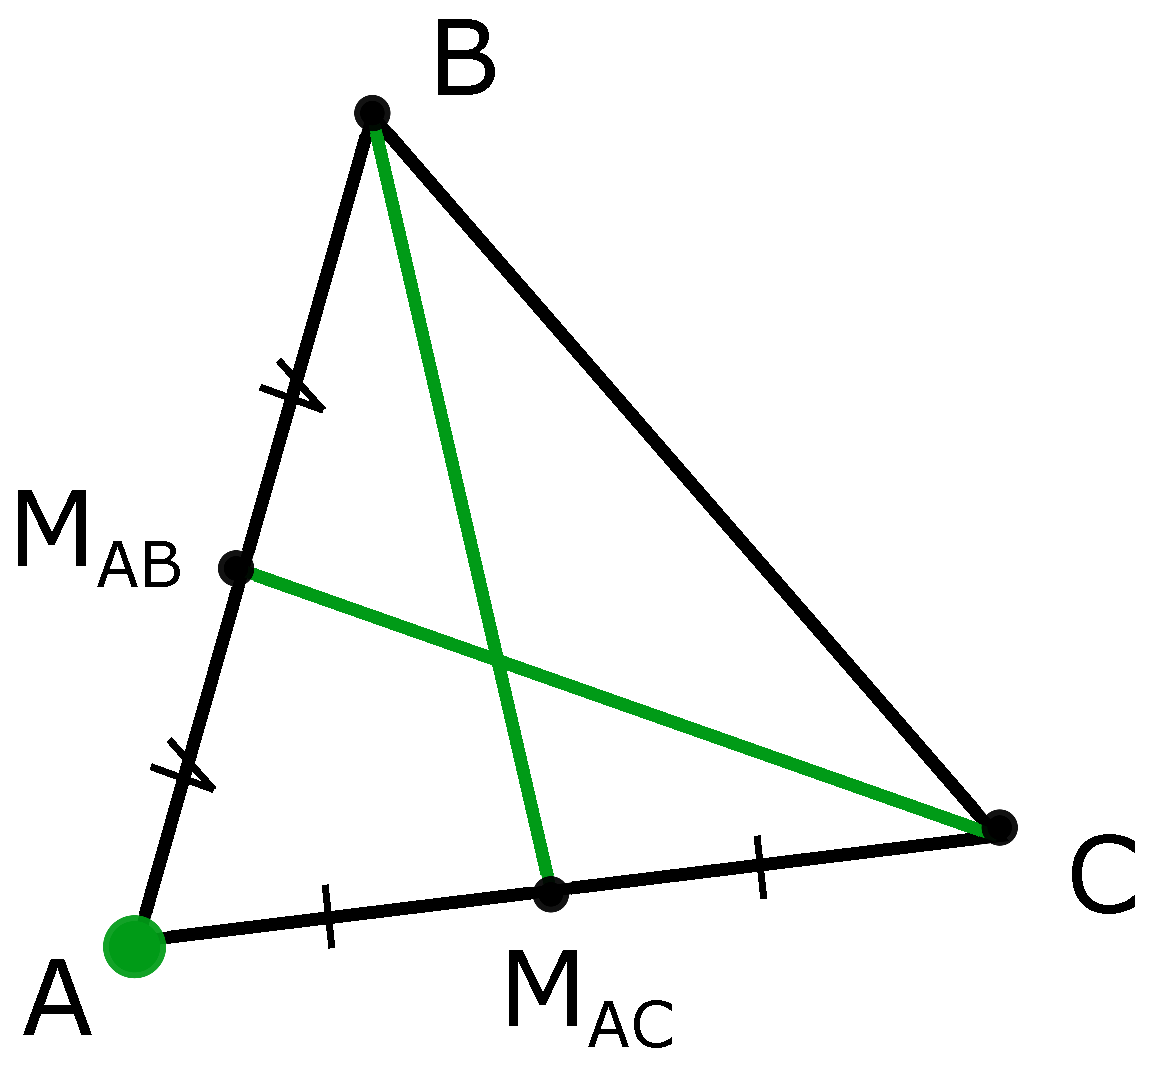
\includegraphics[width=0.75\textwidth]{5-17}
    \end{figure}
  \end{frame}
    
    
  \begin{frame}{\# 5.17}
    \begin{block}{Решение}
      Координаты вершин: $A(1, 1), B(12, -9), C(11, -7)$
      
      \pause
      
      \begin{enumerate}
        \setcounter{enumi}{4}
        
        \item Уравнение прямой $AB$:
        \[
          \widetilde A_{AB} x + \widetilde B_{AB} y + \widetilde C_{AB} = 0
        \]
        \[
          \left\{
            \begin{aligned}
              &\widetilde A_{AB} + \widetilde B_{AB} + \widetilde C_{AB} = 0\\
              &12 \widetilde A_{AB} -9 \widetilde B_{AB} + \widetilde C_{AB} = 0
            \end{aligned}
          \right.
          \Rightarrow
          \left\{
            \begin{aligned}
              &\widetilde A_{AB} = -\frac{10}{21}\widetilde C_{AB}\\
              &\widetilde B_{AB} = -\frac{11}{21}\widetilde C_{AB}
            \end{aligned}
          \right.
        \]
        \[
          -10x - 11y + 21 = 0
        \]
        
        \item Аналогично для сторон $BC$, $AC$.
      \end{enumerate}
    \end{block}
  \end{frame}
    
    
  \section{\uline{5.19}}
  
  \begin{frame}{\# 5.19}
  
    % TODO: добавить везде про систему координат

    \begin{block}{Условие}
      Составить уравнения прямых, проходящих через точку $A(-1, 5)$ и равноудалённых от точек $B(3, 7)$ и $C(1, -1)$.
    \end{block}
    
    \pause
    
    \begin{block}{\only<2>{Решение}\only<3>{\sout{Решение}}}
      Расстояние от точки до прямой:
      $\rho = \frac{\bigl|(\bds r_1 - \bds r_0, \bds n)\bigr|}{|\bds n|}$
      
      Прямая $a$ равноудалена от $B(3, 7)$ и $C(1, -1)$:
      \[
        \frac{\Bigl|\bigl((3, 7) - (-1, 5), \bds n\bigr)\Bigr|}{|\bds n|} = \rho_{a, B}
        = \rho_{a, C}
        = \frac{\Bigl|\bigl((1, -1) - (-1, 5), \bds n\bigr)\Bigr|}{|\bds n|}
      \]
      
      \pause
      
      Но система координат не прямоугольная!
      \begin{equation*}
      \begin{split}
        (\bds u, \bds v)
        &= (x_u \bds e_1 + y_u \bds e_2, x_v \bds e_1 + y_v \bds e_2)\\
        &= x_u x_v(\bds e_1, \bds e_1) + y_u y_v(\bds e_2, \bds e_2) + (x_u y_v + y_u x_v)(\bds e_1, \bds e_2)
      \end{split}
      \end{equation*}
    \end{block}
  \end{frame}
    
    
  \begin{frame}{\# 5.19}
    \begin{figure}
      \centering
      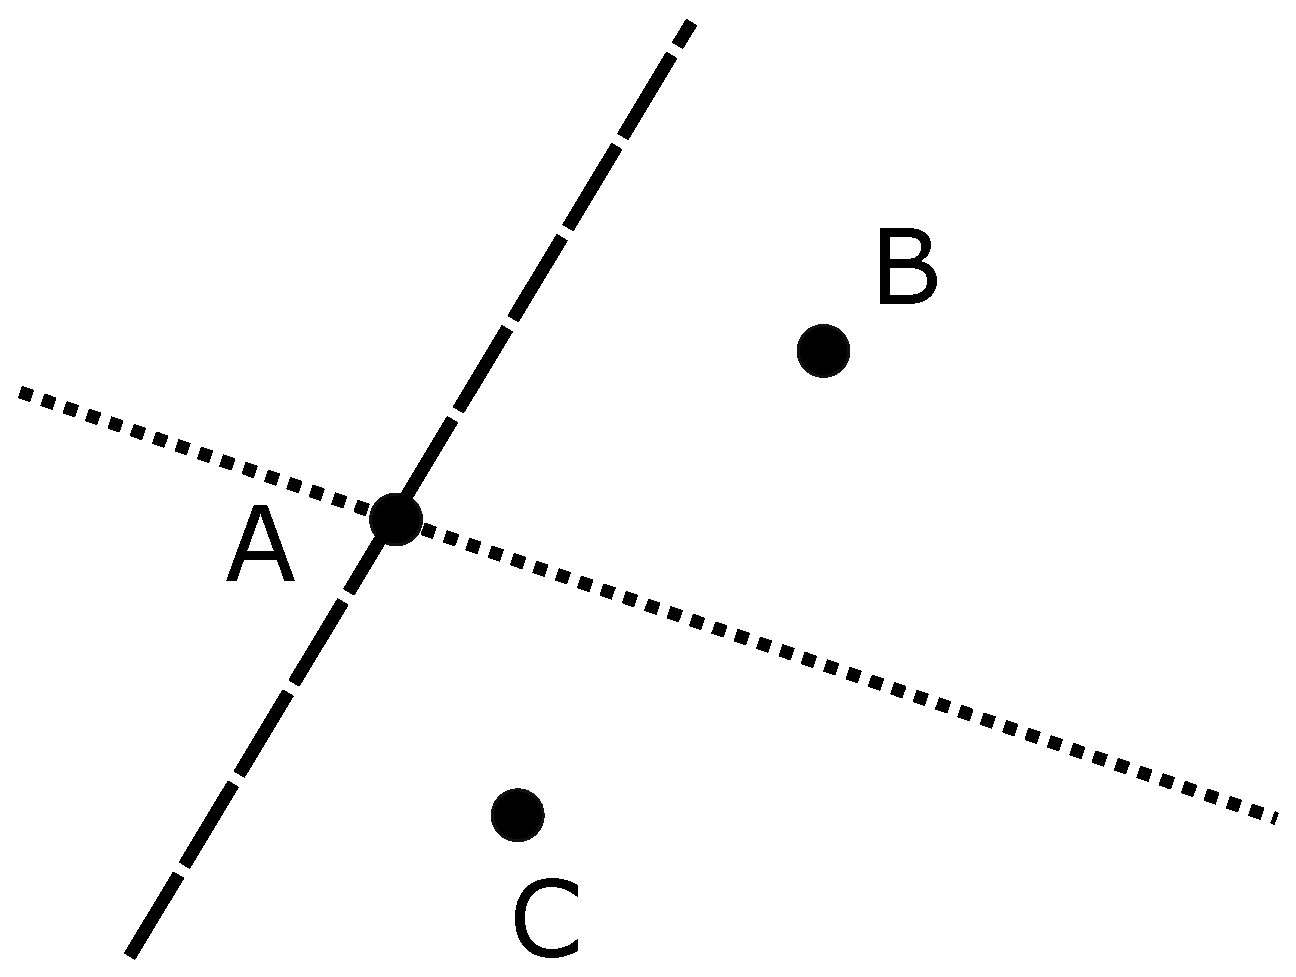
\includegraphics[width=0.75\textwidth]{5-19}
    \end{figure}
  \end{frame}
    
  \begin{frame}{\# 5.19}
    % TODO: picture
    \begin{block}{Решение}
      \begin{enumerate}
        \item Прямая $a$ параллельна $\bds{BC} \hm= (1 - 3, -1 - 7) \hm= (\textcolor{my-blue}{-2}, \textcolor{my-red}{-8})$:
        \[
          a: \textcolor{my-red}{-8} x - \textcolor{my-blue}{(-2)} y + C = 0
        \]
        \[
          A \in a \Rightarrow -8 \cdot (-1) + 2 \cdot 5 + C = 0 \Rightarrow C = -18
        \]
        \[
          \boxed{4x - y + 9 = 0}
        \]
        
        \pause
        
        \item Прямая $a$ проходит между точками $B$ и $C$.
        
        Пусть $M$~---~середина $BC$:
        $
          M = \left(\frac{1 + 3}{2}, \frac{-1 + 7}{2}\right) = (2, 3)
        $
        
        Прямая, проходящая через две точки $A(-1, 5)$ и $M(2, 3)$:
        \[
          \frac{x - x_M}{x_A - x_M} = \frac{y - y_M}{y_A - y_M}
          \Rightarrow
          \frac{x - 2}{-1 - 2} = \frac{y - 3}{5 - 3}
        \]
        \[
          \boxed{2x + 3y - 13 = 0}
        \]
      \end{enumerate}
    \end{block}
  \end{frame}
    
    
  \section{5.34(2) (р)}
  
  \begin{frame}{\# 5.34(2) (р)}
    \begin{block}{Условие}
      Точка $A(1, 2)$ и прямая $a: 3x - y + 9 = 0$.
      Найти координаты
      \begin{enumerate}
        \item $A_{\perp}$~---~проекции $A$ на прямую $a$
        \item $A'$~---~точки, симметричной с $A$ относительно прямой $a$
      \end{enumerate}
    \end{block}
    
    \pause
    
    \begin{block}{Решение}
      \begin{enumerate}
        \item Точка $A$ не лежит на прямой: $3 \hm\cdot 1 \hm- 1 \hm\cdot 2 \hm+ 9 \hm{\not=0}$
        
        \pause
        
        \item Система прямоугольная $\Rightarrow \bds n \hm= (3, -1)$.
        
        \pause
        
        \item $A_{\perp} \hm=(x, y)$, $A_{\perp} \in a$, $\bds{A_{\perp}A} \hm\parallel \bds n$:
        \[
          \left\{
            \begin{aligned}
              &3x - y + 9 = 0\\
              &\frac{1 - x}{2 - y} = \frac{x_A - x_{A_{\perp}}}{y_A - y_{A_{\perp}}} = \frac{n_x}{n_y} = \frac{3}{-1}
            \end{aligned}
          \right.
        \]
        \[
          \boxed{A_{\perp} = (-2, 3)}
        \]
      \end{enumerate}
    \end{block}
  \end{frame}
    

  \begin{frame}{\# 5.34(2) (р)}
    \begin{block}{Решение}
      \begin{enumerate}
        \setcounter{enumi}{3}
    
        \item $A, A_{\perp}, A'$:
        \[
          \left\{\begin{aligned}
            &\bds{AA_{\perp}} = \bds{A_{\perp}A'}\\
            &\bds{AA_{\perp}} = (-2, 3) - (1, 2) = (-3, 1)
          \end{aligned}\right.
          \Rightarrow \bds{A_{\perp}A'} = (-3, 1)
        \]
        \[
          \bds{A_{\perp}A'} = A' - A_{\perp} \Rightarrow A' = \bds{A_{\perp}A'} + A_{\perp}
          = (-3, 1) + (-2, 3)
        \]
        \[
          \boxed{\bds{A_{\perp}A'} = (-5, 4)}
        \]
      \end{enumerate}
    \end{block}
  \end{frame}

    
  \section{\uline{5.53 (р)}}
  
  \begin{frame}{\# 5.53 (р)}
    % Не такое решение, как в задачнике
    
    \begin{block}{Условие}
      Две прямые: $x - 7y = 1$ и $x + y \hm= -7$.
      Угол с точкой $A(1, 1)$ внутри.
      Уравнение биссектрисы?
    \end{block}
    
    \pause
    
    \begin{block}{Решение}
      \begin{enumerate}
        \item Прямые пересекаются, точка $A$ не лежит ни на одной прямой.
        
        \item Точка пересечения прямых $X(x, y)$:
        \[
          \left\{\begin{aligned}
            &x - 7y = 1\\
            &x + y = -7
          \end{aligned}\right.
          \Rightarrow
          \left\{\begin{aligned}
            &x = -6\\
            &y = -1
          \end{aligned}\right.
        \]
        \[
          \boxed{X = (-6, -1)}
        \]
      \end{enumerate}
    \end{block}
  \end{frame}
    

  \begin{frame}{\# 5.53 (р)}
    \begin{figure}
      \centering
      \includegraphics[width=0.75\textwidth]{5-53}
    \end{figure}
  \end{frame}


  \begin{frame}{\# 5.53 (р)}
    \begin{block}{Решение}
      \begin{enumerate}
        \setcounter{enumi}{2}
        % TODO: рисунок
        
        \item Выберем направляющие векторы прямых $\bds{a_1}$, $\bds{a_2}$ так, чтобы они образовывали угол с точкой $A$ внутри.
        \[
          [\bds{a_i}, \vv{XA}] = \left|
            \begin{aligned}
              &\bds i & &\bds j & &\bds k\\
              &a_{ix} & &a_{iy} & &0\\
              &XA_x & &XA_y & &0
            \end{aligned}
          \right|
          = \bds k \cdot (a_{ix} \cdot XA_y - XA_x \cdot a_{iy})
        \]
        \[
          \vv{XA} = (1, 1) - (-6, -1) = (7, 2)
        \]
        \[
          \bds{a_1} = (7, 1) \Rightarrow \sgn{(7 \cdot 2 - 7 \cdot 1)} = +
        \]
        \[
          \bds{a_2} = (-1, 1) \Rightarrow \sgn{(-1 \cdot 2 - 7 \cdot 1)} = -
        \]
        \[
          \boxed{\bds{a_1} = (7, 1),\ \bds{a_2} = (-1, 1)}
        \]
      \end{enumerate}
    \end{block}
  \end{frame}


  \begin{frame}{\# 5.53 (р)}
    \begin{block}{Решение}
      \begin{enumerate}
        \setcounter{enumi}{3}
        % TODO: рисунок
        
        \item Пусть $\bds b \hm= (b_x, b_y)$~---~направляющий вектор биссектрисы. Точки на биссектрисе равноудалены от сторон угла:
        \[
          \frac{(\bds{a_1}, \bds b)}{|\bds{a_1}||\bds b|} = \cos \angle (\bds{a_1}, \bds b)
          = \cos \angle (\bds{a_2}, \bds b)
          = \frac{(\bds{a_2}, \bds b)}{|\bds{a_2}||\bds b|}
        \]
        \[
          \frac{7 b_x + b_y}{|\bds{a_1}|} = \frac{-b_x + b_y}{|\bds{a_2}|}
          \Rightarrow
          \bds b = \bigl(|\bds{a_1}| - |\bds{a_2}|, 7|\bds{a_2}| + |\bds{a_1}|\bigr)
        \]
        \[
          |\bds{a_1}| = \sqrt{50},\ |\bds{a_2}| = \sqrt{2} \Rightarrow \bds b = (5 - 1, 7 + 5) = (4, 12)
        \]
        
        \pause
        
        \item Уравнение биссектрисы:
        \[
          \frac{x - (-6)}{4} = \frac{y - (-1)}{12}
          \Rightarrow \boxed{3x - y + 17 = 0}
        \]
      \end{enumerate}
    \end{block}
  \end{frame}


  \section{5.35}
  
  \begin{frame}{\# 5.35}
    \begin{block}{Условие}
      Составить уравнение прямой, симметричной прямой $a: 3x \hm- y \hm+ 5 \hm= 0$ относительно прямой $l: x \hm+ y \hm- 1 \hm= 0$.
    \end{block}
    
    \pause
    
    \begin{block}{Решение}
      % TODO: picture
      
      \begin{enumerate}
        \item Точка пересечения прямых $X$:
        \[
          \left\{\begin{aligned}
            &3x - y + 5 = 0\\
            &x + y - 1 = 0
          \end{aligned}\right.
          \Rightarrow X = (-1, 2)
        \]
        
        \pause
        
        \item Точка $A$ на прямой $3x - y + 5 = 0$:
        \[
          3 \cdot 0 - 5 + 5 = 0
          \Rightarrow A = (0, 5)
        \]
      \end{enumerate}
    \end{block}
  \end{frame}
    
    
  \begin{frame}{\# 5.35}
    \begin{block}{Решение}
      % TODO: picture
        
      \begin{enumerate}
         \setcounter{enumi}{2}
          
          \item Проекция $\pi_{\vv{XA}}$ вектора $\vv{XA} \hm= (1, 3)$ на прямую $l$ с направляющим вектором $\bds l = (-1, 1)$:
          \[
            \pi_{\vv{XA}} = \vv{XA} \cdot \cos \angle(\vv{XA}, l)
            = \frac{(\vv{XA}, \bds l)}{|\bds l|}
            = (1, 3) \cdot \frac{1}{\sqrt 2} (-1, 1)
            = \sqrt 2
          \]
          
          \pause
          
          \item Проекция $\pi_A$ точки $A$ на $l$:
          \[
            \pi_A = X + \frac{\bds l}{l} \cdot \pi_{\vv{XA}}
            = (-1, 2) + (-1, 1) = (-2, 3)
          \]
          
          \pause
          
          \item Точка $A'$, симметричная точке $A$ относительно $l$:
          \[
            A' = \pi_A + \bigl(\pi_A - A\bigr) = (-4, 1)
          \]
      \end{enumerate}
    \end{block}
  \end{frame}
        

  \begin{frame}{\# 5.35}
    \begin{block}{Решение}
      % TODO: picture
      
      \begin{enumerate}
       \setcounter{enumi}{5}
        
        \item Прямая, проходящая через две точки $X(-1, 2)$ и $A'(-4, 1)$:
        \[
          \frac{x - (-1)}{y - 2} = \frac{-4 - (-1)}{1 - 2}
          \Rightarrow
          \boxed{x - 3y + 7 = 0}
        \]
      \end{enumerate}
    \end{block}
  \end{frame}
\end{document}
